\chapter{Tahapan Membuat Aplikasi Akademik Sederhana Oracle Apex}

\section{Membuat Tabel Di Microsoft Excel Dan Normalisasi Tabel}
\begin{enumerate}
    \item Membuat sebauh tabel pada excel. Contoh Disini menggunakan tabel dari modul basis data 1. Terdapat tabel Mahasiswa, Dosen, Kuliah, Nilai, dan Jadwal. Pada tabel Dosen, Nilai, dan jadwal masih kurang tepat, maka dilakukan normalisasi pada tabel tersebut.\par
    - Tabel sebelum normalisasi
    
    \begin{figure}[!htbp]
        \centering
        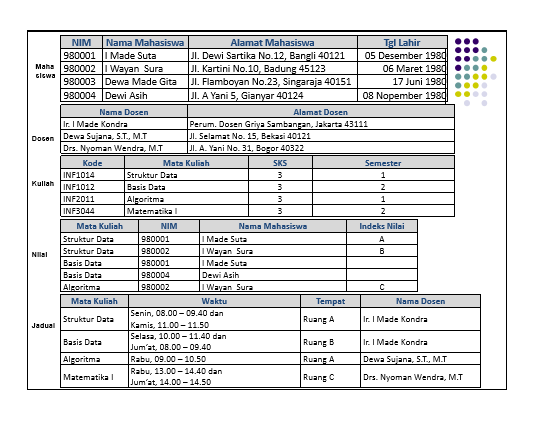
\includegraphics[scale=0.7]{figure/tabel_sebelum_normalisasi.PNG}
        \caption{\textit{tabel sebelum normalisasi}}
        \label{fig:my_label}
    \end{figure}
    
    \par 
    
    - Tabel dosen sesudah normalisai. Pada tabel dosen, ditambahkan NIK sebagai Primary key.\par
    
    \newpage
    \begin{figure}[!htbp]
        \centering
        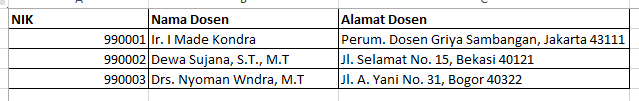
\includegraphics[scale=0.7]{figure/tabel_dosen.PNG}
        \caption{\textit{tabel dosen}}
        \label{fig:my_label}
    \end{figure}\par
    
    - Tabel nilai sesudah normalisasi. Di tabel nilai sebelumnya, terdapat atribut mata kuliah. Atribut tersebut diganti dengan hanya memasukkan kode mata kuliah / primary key dari mata kuliah. Dan pada tabel sebelumnya juga terdapat atribut nama mahasiswa, cukup dengan menggunakan NIM/primary key dari mahasiswa saja, sehingga atribut nama mahasiswa dihapuskan.\par
    
    \begin{figure}[!htbp]
        \centering
        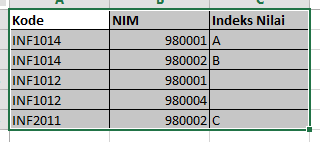
\includegraphics[scale=0.7]{figure/tabel_nilai.PNG}
        \caption{\textit{tabel nilai}}
        \label{fig:my_label}
    \end{figure}\par
    
    - Tabel jadwal sesudah normalisasi. Sama dengan tabel nilai, di tabel jadwal juga terdapat atribut mata kuliah. Atribut tersebut diganti dengan hanya memasukkan kode mata kuliah / primary key dari mata kuliah. Nah selanjutnya ada atribut dosen yang diganti dengan atribut NIK.\par
    
    \begin{figure}[!htbp]
        \centering
        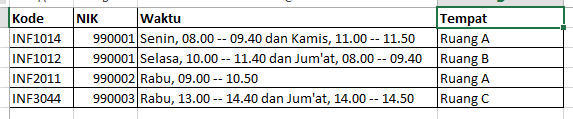
\includegraphics[scale=0.7]{figure/tabel_jadwal.PNG}
        \caption{\textit{tabel jadwal}}
        \label{fig:my_label}
    \end{figure}
    \end{enumerate}
    
\section{Memasukkan Tabel Di Microsoft Excel Ke Oracle Apex}

\begin{enumerate}
    \item Setelah tabel sudah siap, selanjutnya login ke akun Oracle Apex Online
    
    \begin{figure}[!htbp]
        \centering
        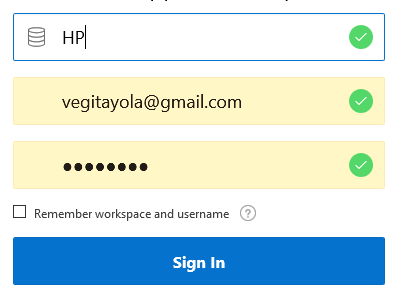
\includegraphics[scale=0.5]{figure/login_oracle_apex.PNG}
        \caption{\textit{login oracle apex}}
        \label{fig:my_label}
    \end{figure}
    
    \newpage
    \item Pilih app builder dan create
    
    \begin{figure}[!htbp]
        \centering
        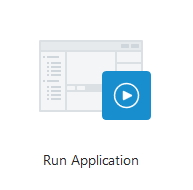
\includegraphics[scale=0.5]{figure/run_app.PNG}
        \caption{\textit{run app}}
        \label{fig:my_label}
    \end{figure}
    
    \begin{figure}[!htbp]
        \centering
        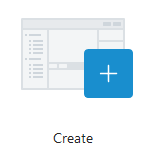
\includegraphics[scale=0.5]{figure/create.PNG}
        \caption{\textbf{create}}
        \label{fig:my_label}
    \end{figure}
    
    \item Pilih From a File, Untuk memasukkan file atau tabel yang telah kita buat tadi yakni dalam bentuk exel. Dan pilih file.
    
    \begin{figure}[!htbp]
        \centering
        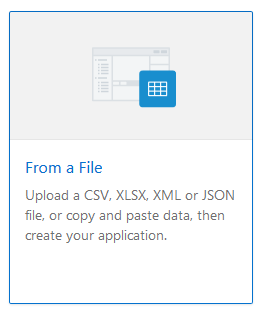
\includegraphics[scale=0.5]{figure/from_a_file.PNG}
        \caption{\textit{from a file}}
        \label{fig:my_label}
    \end{figure}
    
    \begin{figure}[!htbp]
        \centering
        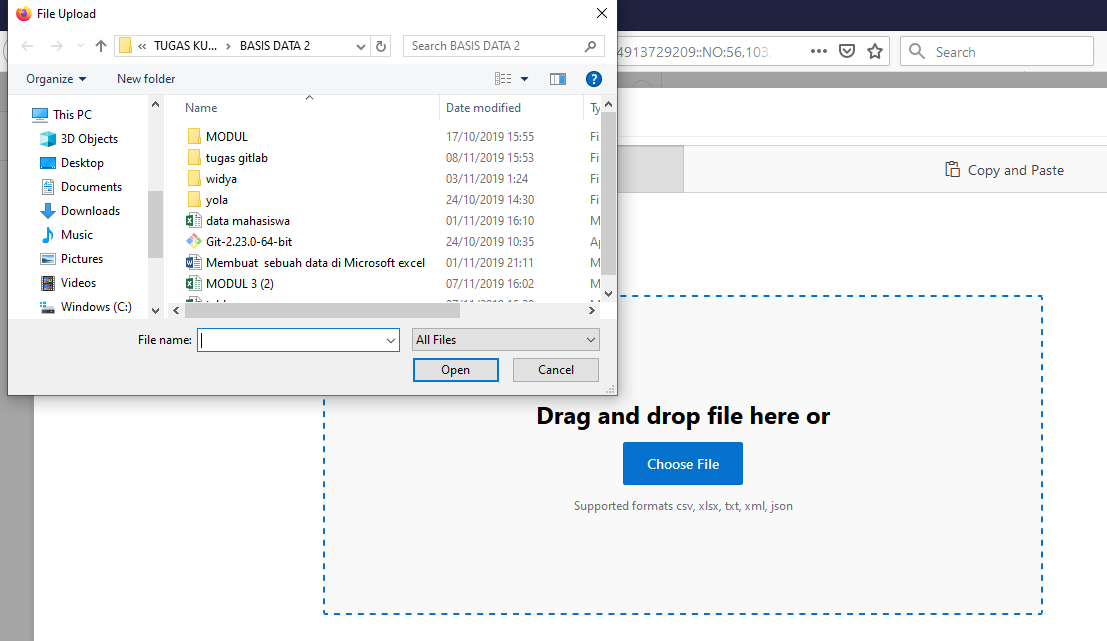
\includegraphics[scale=0.5]{figure/choose_file.PNG}
        \caption{\textit{choose file}}
        \label{fig:my_label}
    \end{figure}
    
    \newpage
    \item Beri nama sesuai urutan tabel tadi, dari yang pertama beri nama tabel Maha- siswa,pastikan select sheet nya sesuai dengan penamaan tabelnya. Selanjutnya Load data. Lakukan hal yang sama pada tabel yang selanjutnya.
    
    \begin{figure}[!htbp]
        \centering
        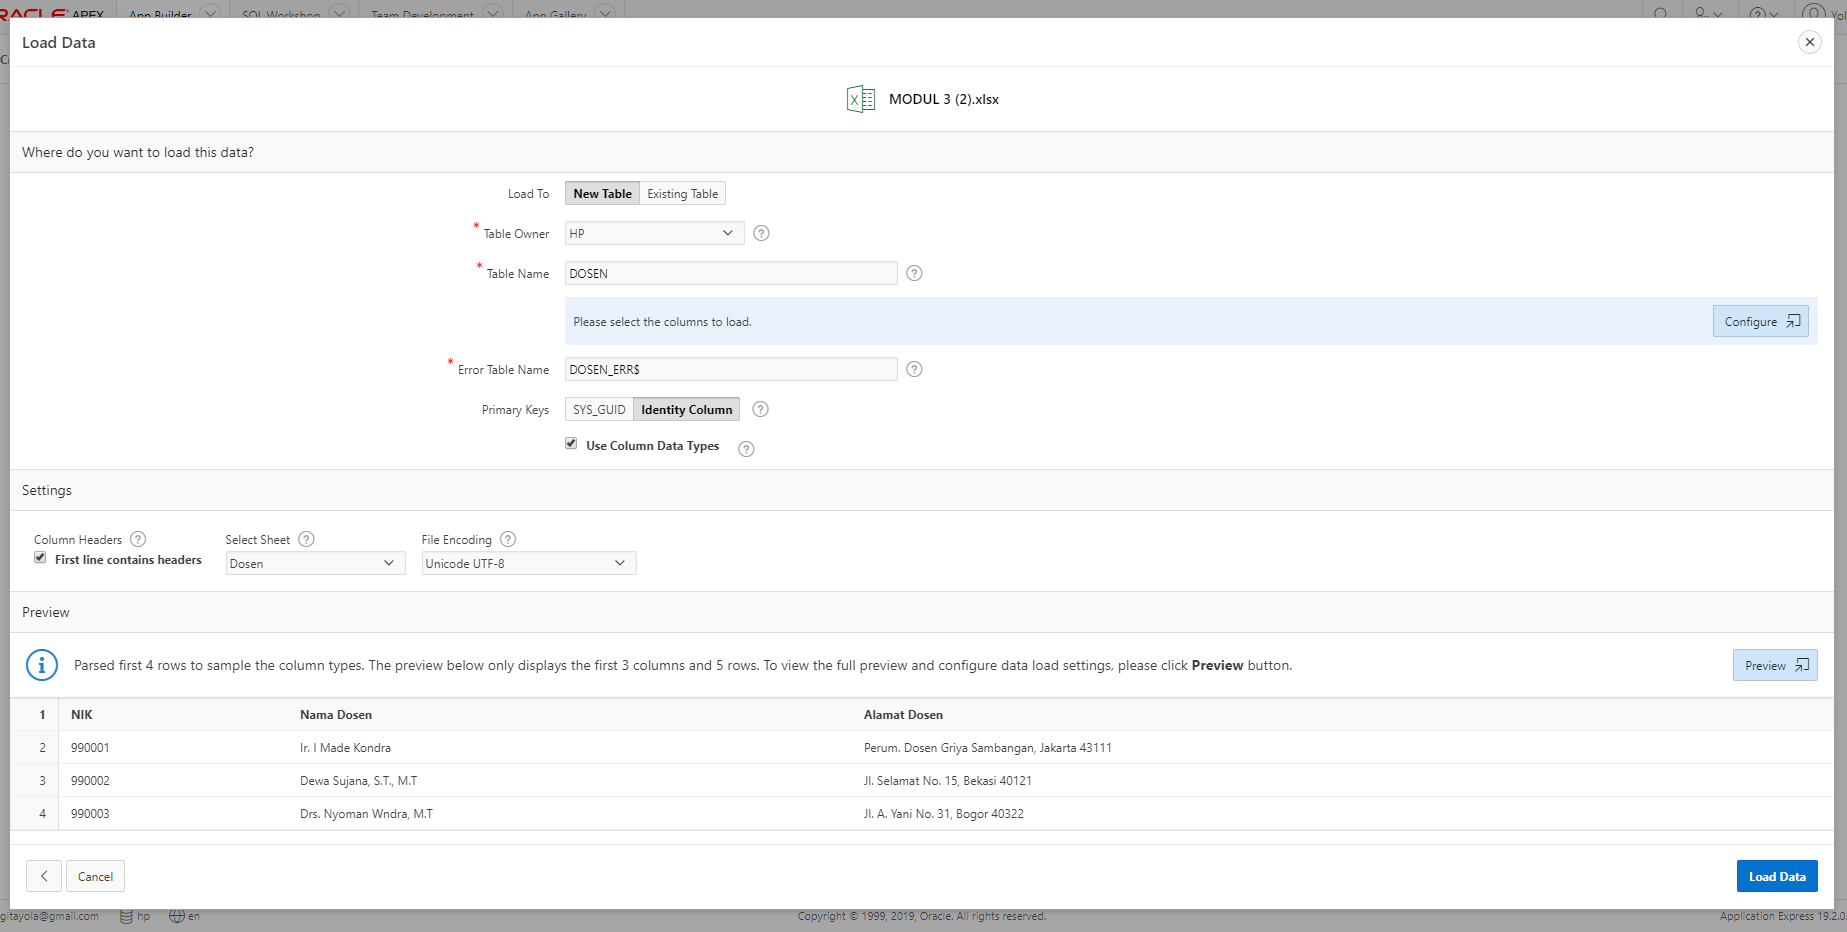
\includegraphics[scale=0.3]{figure/pemilihan_dan_beri_nama_tabel.PNG}
        \caption{\textit{pemilihan dan beri nama tabel}}
        \label{fig:my_label}
    \end{figure}
    
    \item Berikut tampilan tabel yang telah kita buat
    
    \begin{figure}[!htbp]
        \centering
        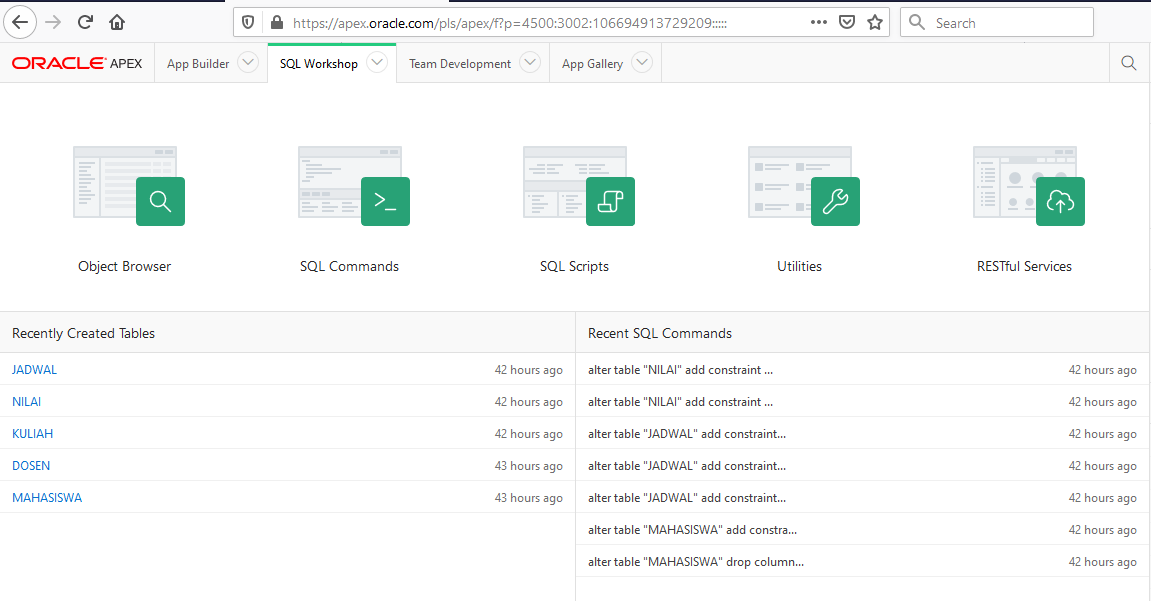
\includegraphics[scale=0.5]{figure/tampil_tabel.PNG}
        \caption{tampil tabel}
        \label{fig:my_label}
    \end{figure}{}
\end{enumerate}

\section{Membuat Primary Key}

\begin{enumerate}
    \item 1.	Masuk ke object browser. Nah proses selanjutnya adalah menentukan primary key dan foreign key. sebelum membuat foreign key, terlebih dahulu kita membuat primary keynya. Klik tabel yang akan dibuat primary key. klik constraints, lalu create. Setelah itu ubah type constranint menjadi primery key. dan yang terakhir, tentukan atribut yang dijadikan primary key.
    
    \begin{figure}[!htbp]
        \centering
        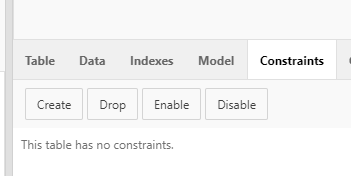
\includegraphics[scale=0.7]{figure/constraints.PNG}
        \caption{\textit{constraints}}
        \label{fig:my_label}
    \end{figure}
    
    \begin{figure}[!htbp]
        \centering
        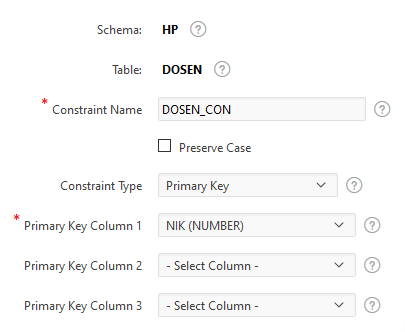
\includegraphics[scale=0.7]{figure/primary_key.PNG}
        \caption{\textit{primary key}}
        \label{fig:my_label}
    \end{figure}
    
    \newpage
    \item Berikut ini tampilan apabila primary key telah berhasil dibuat
    
    \begin{figure}[!htbp]
        \centering
        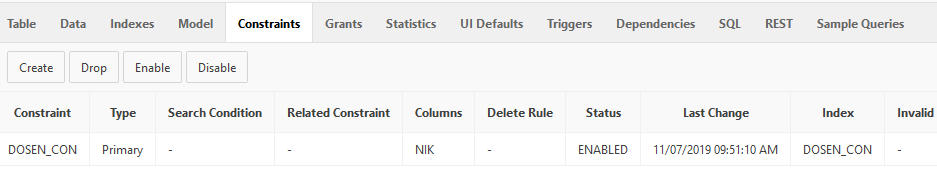
\includegraphics[scale=0.7]{figure/tabel_yang_sudah_ada_primary_key.PNG}
        \caption{\textit{tabel yang sudah ada primary key}}
        \label{fig:my_label}
    \end{figure}\par
    
    Satu tabel hanya dapat memiliki satu primary key.  lanjutkan pembuatan primary key ke tabel Mahasiswa dengan primary keynya NIM, Dosen dengan primary keynya NIK, dan Kuliah dengan primary keynya Kode.\par
    
\end{enumerate}

\section{Membuat Foreign Key}

\begin{enumerate}
    \item Membuat foreign key. Apabila sebuah tabel memiliki atribut yang menjadi primary key di tabel lain, maka atribut tersebut menjadi foreign key. membuat foreign key, klik constraints dan create. lalu ubah type constraints menjadi foreign key. 
    
    \newpage
    \begin{figure}[!htbp]
        \centering
        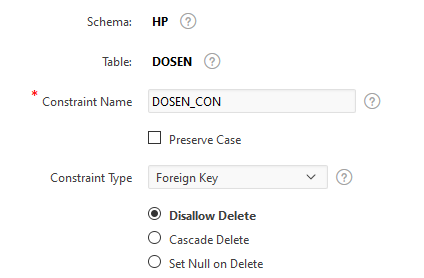
\includegraphics[scale=0.7]{figure/foreign_key.PNG}
        \caption{\textit{foreign key}}
        \label{fig:my_label}
    \end{figure}
    
    \item Pilih atribut yang menjadi primary key di tabel lain. Pilih juga tabel asal dari atribut tersebut.
    
    \begin{figure}[!htbp]
        \centering
        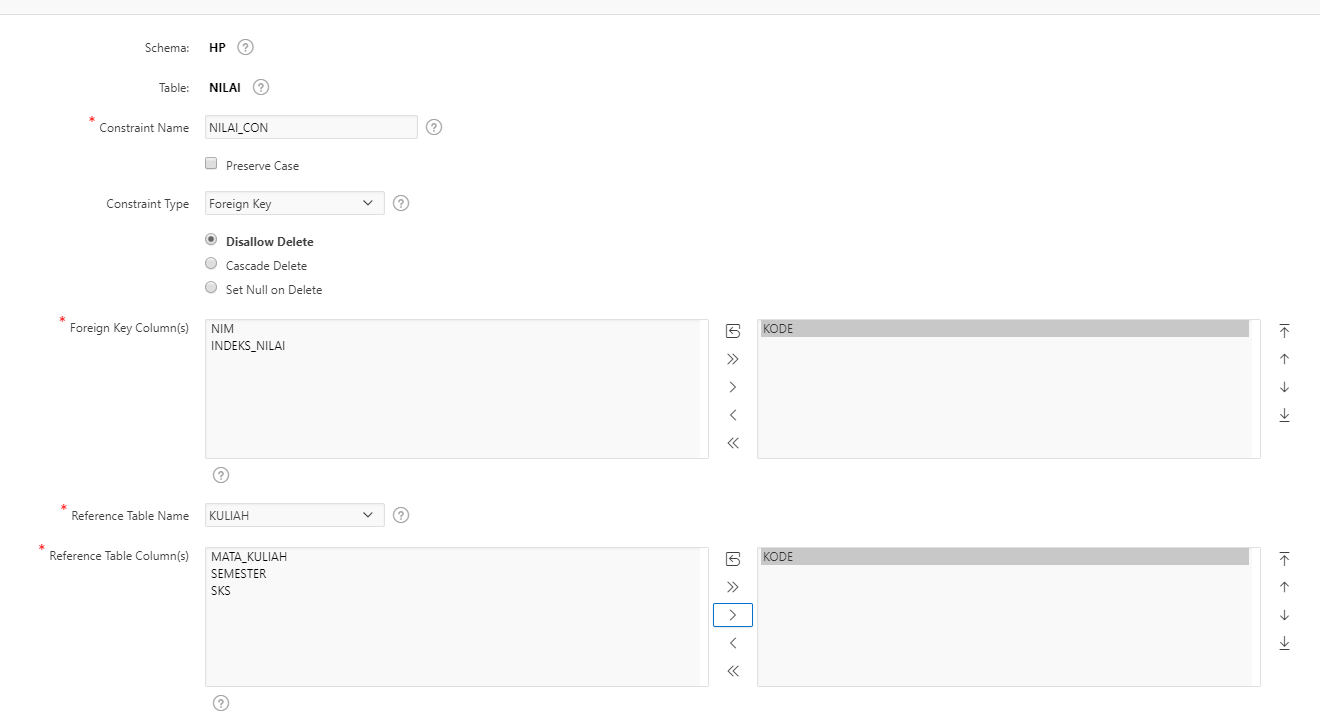
\includegraphics[scale=0.5]{figure/pengaturan_foreign_key.PNG}
        \caption{\textit{pengaturan foreign key}}
        \label{fig:my_label}
    \end{figure}
    
    \item Apabila dalam sebuah tabel memiliki lebih dari satu foreign key, dibuat dengan nama yang berbeda.
    
    \newpage
    \begin{figure}[!htbp]
        \centering
        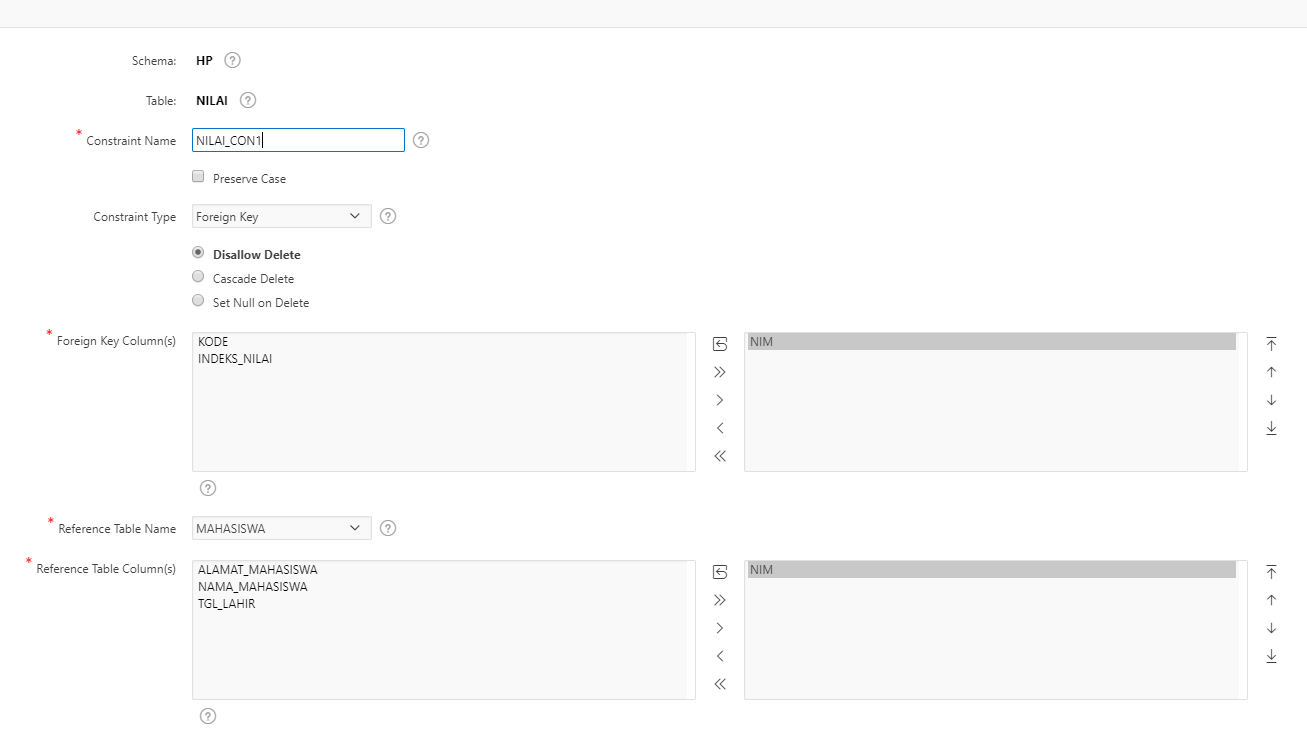
\includegraphics[scale=0.5]{figure/pengaturan_foreign_key_2.PNG}
        \caption{\textit{pengaturan foreign key 2}}
        \label{fig:my_label}
    \end{figure}
    
    \item Berikut tampilan apabila foreign key telah berhasil dibuat
    
    \begin{figure}[!htbp]
        \centering
        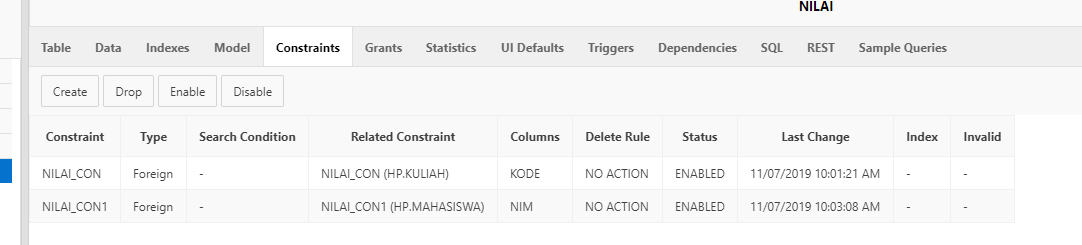
\includegraphics[scale=0.7]{figure/tampilan_tabel_yang_sudah_ada_foreign_key.PNG}
        \caption{\textit{tampilan tabel yang sudah ada foreign key}}
        \label{fig:my_label}
    \end{figure}
    
    Lakukan hal ini ke tabel yang memiliki foreign key.
    
\end{enumerate}

\section{Membuat Aplikasi}

\begin{enumerate}
    \item Klik app builder, lalu klik create. pilih new application
    \newpage
    \begin{figure}[!htbp]
        \centering
        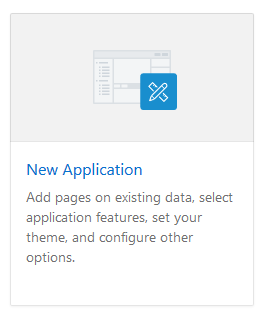
\includegraphics[scale=0.7]{figure/new_aplication.PNG}
        \caption{\textit{new aplication}}
        \label{fig:my_label}
    \end{figure}
    
    \item Klik add page untuk membuat fitur pada applikasi
    
    \begin{figure}[!htbp]
        \centering
        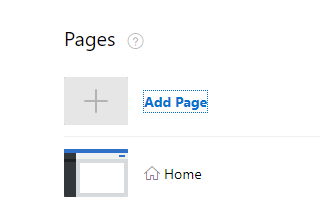
\includegraphics[scale=0.7]{figure/add_page.PNG}
        \caption{\textit{add page}}
        \label{fig:my_label}
    \end{figure}\par
    
    Berikut pilihan pagenya\par
    
    \begin{figure}[!htbp]
        \centering
        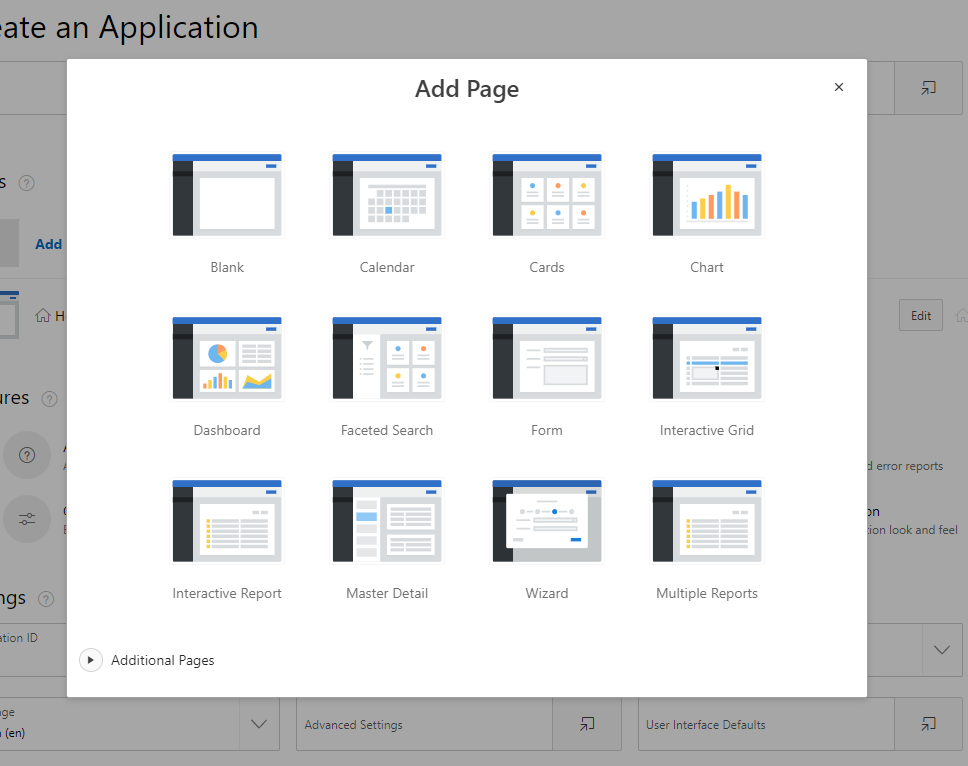
\includegraphics[scale=0.7]{figure/page.PNG}
        \caption{\textit{page}}
        \label{fig:my_label}
    \end{figure}
    
    \newpage
    \item Untuk membuat tabel gunakan Interactive Repot. Berinama tabel Mahasiswa seperti gam- bar dibawah ini. Begitu juga dengan Dosen, Kuliah, Nilai dan Jadwal. Selanjutnya Create Application, jangan lupa memberi nama aplikasi yang ingin kita buat ini.
    
    \begin{figure}[!htbp]
        \centering
        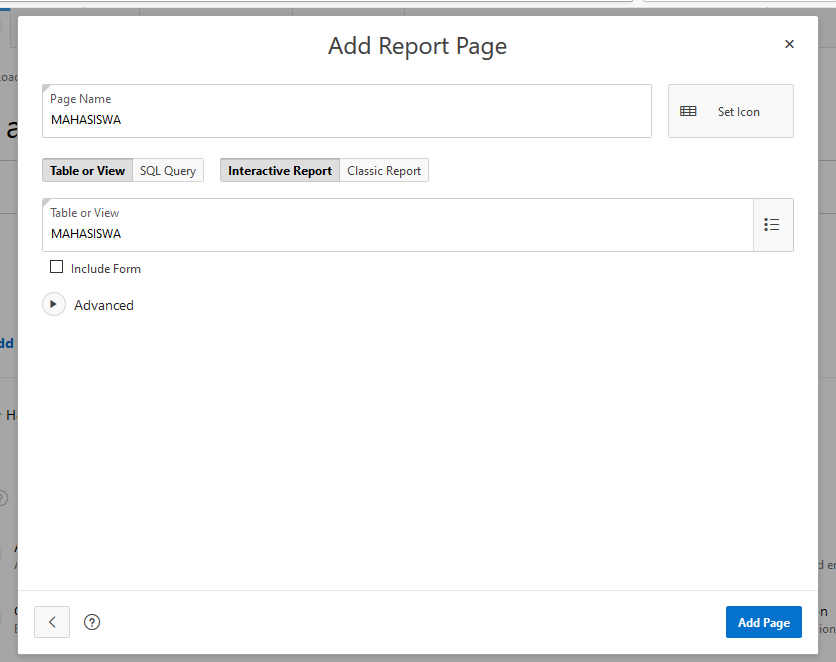
\includegraphics[scale=0.4]{figure/Capture_14_REPORT_PAGE.PNG}
        \caption{\textit{report page}}
        \label{fig:my_label}
    \end{figure}
    
    \item Contoh fitur laiinya adalah dashboard dan master detail.
    
    \begin{figure}[!htbp]
        \centering
        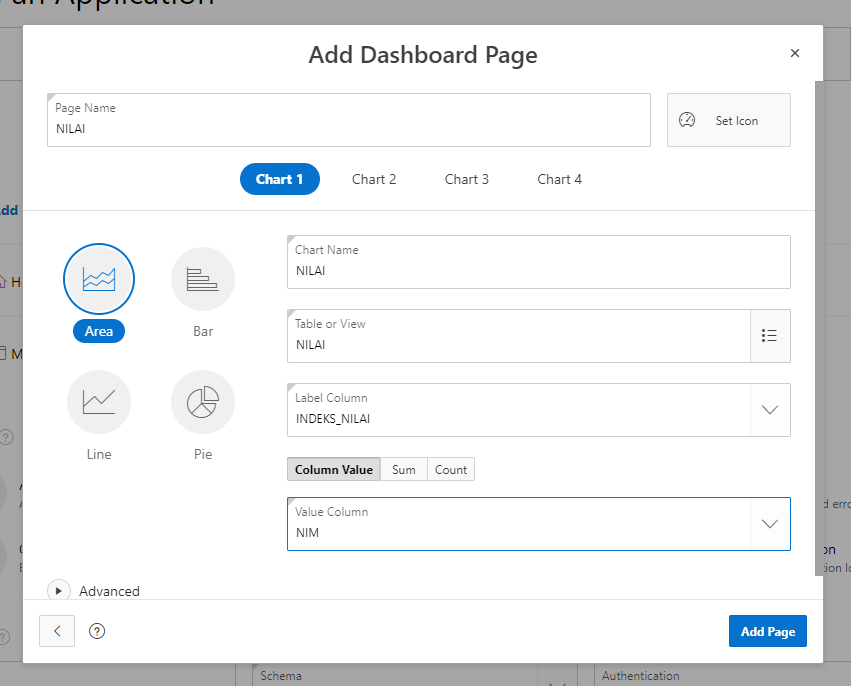
\includegraphics[scale=0.4]{figure/Capture_13_DASHBOARD.PNG}
        \caption{\textit{dashboard page}}
        \label{fig:my_label}
    \end{figure}
    
    \begin{figure}[!htbp]
        \centering
        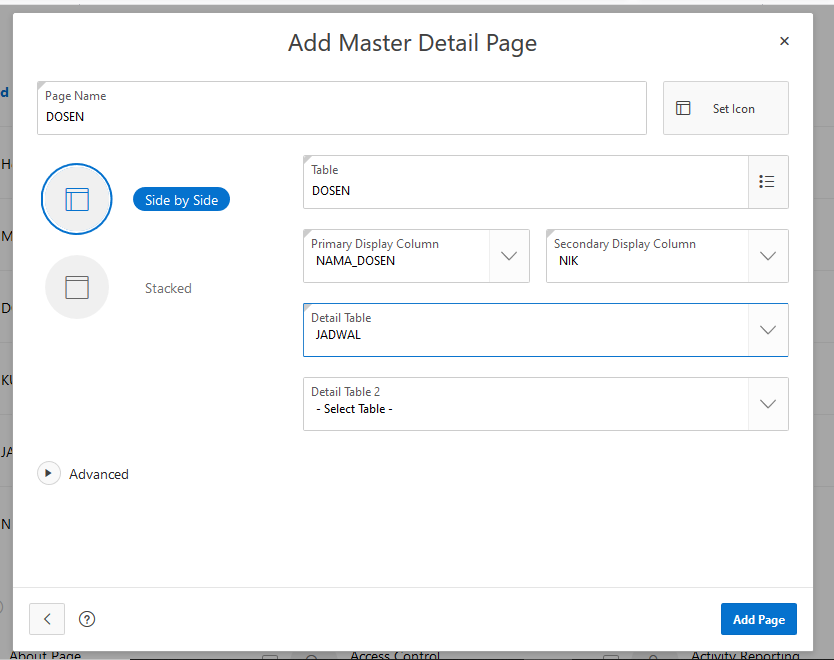
\includegraphics[scale=0.4]{figure/Capture_15_MASTER_DETAIL.PNG}
        \caption{\textit{master detail}}
        \label{fig:my_label}
    \end{figure}
    
    \newpage
    \item Jika semua fitur yang dibutuhkan sudah cukup, Klik create aplikasi
    
   \begin{figure}[!htbp]
       \centering
       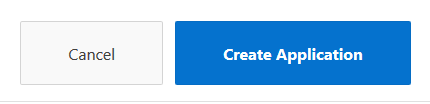
\includegraphics[scale=0.7]{figure/create_app.PNG}
       \caption{\textit{create app}}
       \label{fig:my_label}
   \end{figure}
   
   \item Untuk meilihat aplikasi yang sudah dibuat, klik run app. Dan kemudian login ke akun yang kita miliki.
   
   \begin{figure}[!htbp]
       \centering
       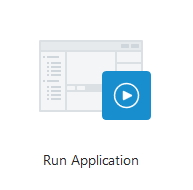
\includegraphics[scale=0.7]{figure/run_app.PNG}
       \caption{\textit{run app}}
       \label{fig:my_label}
   \end{figure}
   
    \newpage
   \begin{figure}[!htbp]
       \centering
       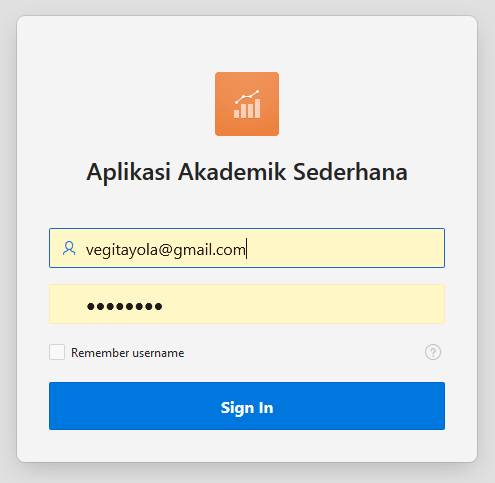
\includegraphics[scale=0.4]{figure/login_akun_app.PNG}
       \caption{\textit{login orecle akun}}
       \label{fig:my_label}
   \end{figure}
   
   \item Berikut tampilan aplikasi yang sduah dibuat
   
   \begin{figure}[!htbp]
       \centering
       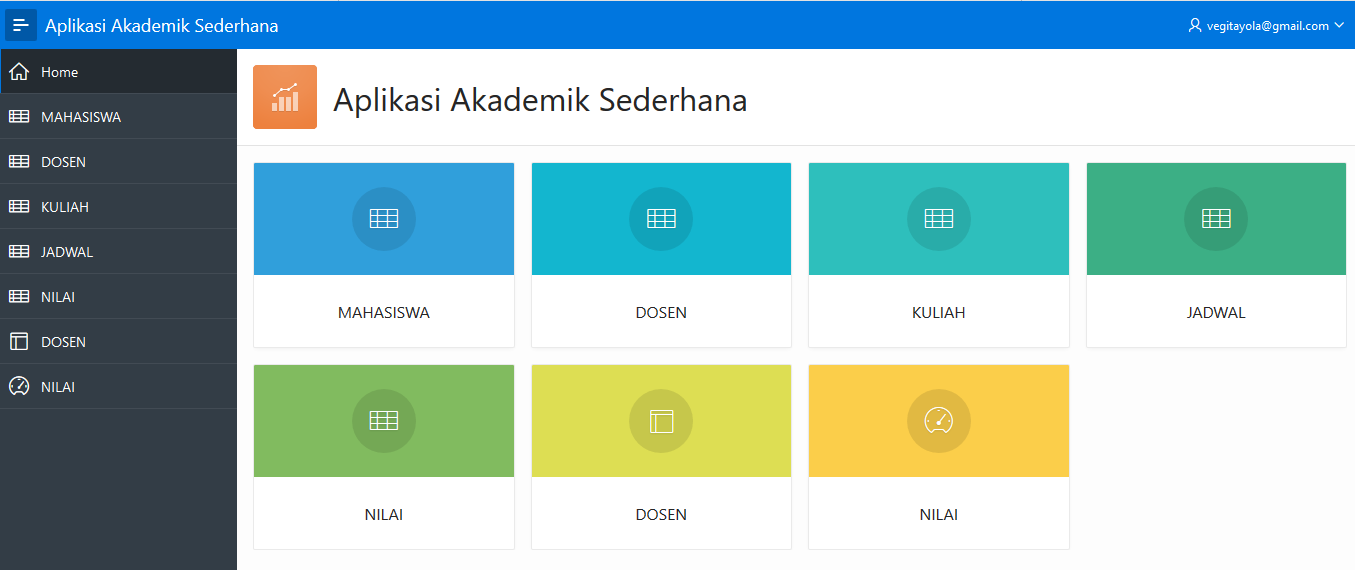
\includegraphics[scale=0.6]{figure/tampilan_app.PNG}
       \caption{\textit{tampilan app}}
       \label{fig:my_label}
   \end{figure}
\end{enumerate}












